%-------------------------------- Configurações --------------------------------

\documentclass[a4paper,         % Tamanho do papel: A4
                 abntfigtabnum,
                 noindentfirst,
                 normaltoc,
                 pnumplain,
                 notimes
                 % capchap,
]{abnt}

% Links border color
\newcommand{\bc}{NavyBlue}
\usepackage{booktabs}% http://ctan.org/pkg/booktabs
\newcommand{\tabitem}{~~\llap{\textbullet}~~}
\usepackage[utf8]{inputenc} % para pode escrever caracteres acentuados normalmente
\usepackage[brazil]{babel}
\usepackage{graphicx}
\usepackage[usenames,dvipsnames]{xcolor} % http://en.wikibooks.org/wiki/LaTeX/Colors
\usepackage[pdfborder={0 0 0},pdfborderstyle={/S/U/W 0.5},citebordercolor=\bc,filebordercolor=\bc,urlbordercolor=\bc,linkbordercolor=\bc]{hyperref} % http://www.tug.org/applications/hyperref/manual.html e http://migre.me/7FH3e
\usepackage[alf]{abntcite}
\usepackage{textcomp}
\usepackage{lineno}
\usepackage{nomencl} % para criar a lista de siglas
\usepackage{lscape} % para usar páginas em landscape (deitadas)
\usepackage{hyperref}
\usepackage{caption}
\usepackage{minted}

\renewcommand\listingscaption{Código}

%------------------------- Numerar subsubsection -------------------------------

\makeatletter
\newcommand\sparagraph{\@startsection{section}{1}{\z@}%
                                    {3.25ex \@plus1ex \@minus.2ex}%
                                    {-1em}%
                                    {\normalfont\normalsize\bfseries}}
\newcommand\ssparagraph{\@startsection{subsection}{2}{\z@}%
                                    {3.25ex \@plus1ex \@minus.2ex}%
                                    {-1em}%
                                    {\normalfont\normalsize\bfseries}}
\newcommand\sssparagraph{\@startsection{subsubsection}{3}{\z@}%
                                    {3.25ex \@plus1ex \@minus.2ex}%
                                    {-1em}%
                                    {\normalfont\normalsize\bfseries}}
\setcounter{secnumdepth}{3}% Allow numbering up to \subsubsection or \sssparagraph
\makeatother

%----------------------- Quebra de linha após paragraph ------------------------

\makeatletter
\renewcommand\paragraph{\@startsection{paragraph}{4}{\z@}%
  {-3.25ex\@plus -1ex \@minus -.2ex}%
  {1.5ex \@plus .2ex}%
  {\normalfont\normalsize\bfseries}}
\makeatother

%--------------------------------- Informações ---------------------------------

\newcommand{\meutitulo}{Modelagem de cloud computing para gerenciamento de recursos computacionais na UENF}

% http://www.tug.org/applications/hyperref/manual.html
\hypersetup{
  pdftitle=\meutitulo,
  pdfauthor=Douglas Oliveira Camata
}

\makenomenclature

\begin{document}

  \titulo{\meutitulo}
  \autor{Douglas Oliveira Camata}
  \instituicao{Universidade Estadual do Norte Fluminense Darcy Ribeiro\par Laboratório de Ciências Matemáticas}
  \orientador[Orientadora:\par]{Profª. Drª. Annabell del Real Tamariz}
  \comentario{Monografia apresentada ao curso de graduação em Ciência da Computação da Universidade Estadual do Norte Fluminense Darcy Ribeiro como requisito para obtenção do título de Bacharel em Ciência da Computação.}
  \local{Campos dos Goytacazes - RJ}
  \data{2014}

  \capa
  \folhaderosto

  \begin{folhadeaprovacao}
  \thispagestyle{empty}
  \center
  \textbf{Douglas Oliveira Camata}
  \vfill

  \center{\textbf{\Large{\textit{\meutitulo}}}}

  \hspace*{2cm}
  \begin{table}[h!]
    \raggedleft
    \begin{tabular}{p{7cm}}
    Monografia apresentada junto ao Curso de Ciência da Computação, da Universidade Estadual do Norte Fluminense Darcy Ribeiro – Campos / RJ, como requisito para obtenção do título de Bacharel em Ciência da Computação.
    Orientadora: Profª. Drª. Annabell del Real Tamariz.
    \end{tabular}
  \end{table}

  \hspace*{2cm}
  \raggedright Aprovado em 25/09/2014.

  \center
  \textbf{COMISSÃO EXAMINADORA}

  \setlength{\ABNTsignthickness}{0.4pt} \setlength{\ABNTsignskip}{1.7cm}

  \assinatura{Profª. Drª. Annabell del Real Tamariz \\ Orientadora - Universidade Estadual do Norte Fluminense Darcy Ribeiro}
  \assinatura{Prof. Dr. Luis Antônio Rivera Escriba \\ Universidade Estadual do Norte Fluminense Darcy Ribeiro}
  \assinatura{Prof. M.Sc. Rodrigo Manhães \\ Universidade Estadual do Norte Fluminense Darcy Ribeiro}
\end{folhadeaprovacao}

  % \begin{titlepage}
 \vspace*{5cm}
 \begin{flushright}
  ``Torna-te aquilo que és.''\\\textit{Friedrich Nietzsche}
  \vspace{1cm}
 \end{flushright}

 \begin{flushright}
  ``(...) me ensino a ser mais tolerante, não julgar ninguém e com isso ser mais feliz (...)''\\\textit{Forfun}
  \vspace{1cm}
 \end{flushright}
\end{titlepage}


  \begin{center}
\textbf{AGRADECIMENTOS} \\ [2.5cm]
\end{center}

À meu pai, meu melhor amigo e grande companheiro, por estar sempre presente em
todos os momentos felizes e tristes da minha vida e por ser a pessoa mais
importante na formação do meu caráter, por eu me tornar quem sou.

À minha mãe e meus irmãos, que mesmo distantes estão sempre por perto e também
são parte da minha motivação.

% À minha namorada Bruna, pelo amor, companheirismo e paciência com a ``mono''.

Aos amigos Eduardo, Tarsis e Hugo, que me convidaram para o \emph{glorioso} NSI,
que foi fundamental para minha formação e meu futuro profissional.

Ao amigos e chefes Rogério, Fábio e Fernando, por estarem sempre no NSI dando
oportunidade e orientando muito bem todos os bolsistas, fazendo acontecer e
puxando a nossa orelha quando necessário.

À todos os companheiros do NSI, desde os mais antigos até os mais novos, por
evoluirmos juntos e posteriormente podermos compartilhar nossos conhecimentos
com os novos bolsistas e sermos reconhecidos e níveis nacional e internacional.

À professora Annabell, pela amizade, pelo ânimo e por confiar na gente na hora
de começar coisas novas e pela paciência para aguentar a todos nós, alunos, durante
todo esse tempo.

À todos meus companheiros de curso, principalmente Eduardo, Thawan e Pedro, por
estarem na luta comigo desde o início de tudo, estudando, se divertindo e,
as vezes, até se dando mal juntos.

À toda minha família, meus avós, meus primos e meus tios, por todo o suporte e
felicidade que me proporcionam sempre.

  \begin{resumo}
O objetivo deste trabalho é apresentar um estudo de caso de um ambiente de \emph{cloud computing},
realizado na Universidade Estadual do Norte Fluminense (UENF), construído através
do conjunto de ferramentas de código livre conhecido como \emph{OpenStack}. Esta
monografia apresenta um apanhado de problemas comuns em instituições públicas, de
ensino e pesquisa com relação a gerencia de seus recuros computacionais, já identificados por
diversos autores, alguns conceitos que servem de base para o \emph{cloud computing}
e como ele pode resolver estes problemas. Também é apresentado um resumo sobre a história
do \emph{OpenStack}, um relato sobre sua instalação, alguns problemas enfrentados
e a interface final que é fornecida para os utilizadores desta \emph{cloud}.
\end{resumo}

  \begin{abstract}
This work intends to present a study of case of a cloud computing environment
in Universidade Estadual do Norte Fluminense (UENF), build using the open-source
tools known as OpenStack. It presents a bunch of common problems in public,
learning and research institutions related to their computational resources
management, already identified by many other authors, some concepts which
serve as base for cloud computing and how it can solve these problems. This
paper also presentes a little briefing of OpenStack's history, a report
about its instalation, the problems encountered, and the final interface
that is provided to the clients of this cloud.
\end{abstract}


  \sumario
  \listoffigures
  \listoftables
  \printnomenclature

  \chapter{Introdução}

Segundo \citeonline{book-cloud-developing-countries}, muitas instituições de ensino superior e pesquisa
de países em desenvolvimento sofrem com diversos problemas relacionados com o gerenciamento dos
seus recursos computacionais. Eles trabalham com grupos que apresentam 3 características:

\begin{itemize}
    \item
        Não possuem acesso adequado aos recursos computacionais para pesquisa e ensino;
    \item
        Se envolvem em alta carga de atividades de ensino;
    \item
        São formados por poucos membros e possuem um orçamento reduzido.
\end{itemize}

Estas atividades (pesquisa e ensino), ainda apresentam outras importantes características.
Por exemplo, elas fazem um grande uso de recursos computacionais em curtos períodos
de tempo, devido à estrutura dos semestres letivos, enquanto outros são usados
mais regularmente \cite{book-cloud-developing-countries}.

Apesar dos avanços em tecnologia, o compartilhamento e gerenciamentos destes recursos
entre instituições de ensino tem recebido uma grande prioridade, principalmente nas
regiões em desenvolvimento \cite{article-sharing-importance}.
\citeonline{article-cloud-developing-countries}
diz ainda que devido às altas demandas de recursos por estas instituições, os grupos dificilmente
conseguem adquirir ou até mesmo manter recursos computacionais de alta performance.

Muitos estudos mostram que \emph{cloud computing} tem benefícios distintos, como
redução de custos, utilização eficiente de recursos computacionais,
flexibilidade e provisionamento elástico \cite{article-cloud-cost-reduction}. Além disso,
\citeonline{book-cloud-developing-countries} diz que todos estes benefícios se aplicam
às duas principais atividades em instituições de ensino superior: pesquisa e ensino. Ele
também diz que existem muitos outros artigos analisando o quão atrativo é o \emph{cloud computing}
para países em desenvolvimento. Ele cita o exemplo de \citeonline{article-cloud-benefits},
que apresenta vários benefícios, como fácil acesso à infraestrutura com baixo custo, melhorando
os esforços para colaboração e o acesso a hardware e softwares mais recentes. Estes benefícios
foram de fato confirmados pelo trabalho de \citeonline{book-cloud-developing-countries}.

Até mesmo instituições governamentais, como o Governo Federal dos Estados Unidos da América,
identificaram \emph{cloud computing} como uma ótima solução para os problemas
que estavam enfrentando que sua estrutura de tecnologia de informação \cite{federal-cloud-computing}.
Estima-se que cerca de 20, dos seus 80 bilhões de dólares de investimento em TI,
serão utilizados para a migração de seus sistemas para este novo paradigma.

\section{Problemática e justificativa}

Segundo \citeonline{article-cloud-developing-countries}, a característica principal
relacionada a pesquisa em instituições de ensino é que os grupos de pesquisa são
pequenos e não são bem coordenados. Como resultado, os investimentos nas pesquisas
acabam sendo \textit{ad-hoc}, sob demanda e muito frequentemente não coordenados. Ainda
dentro deste assunto, o autor diz que estes grupos tendem a resolver problemas pequenos e
que não são recentes, porque não possuem recursos suficientes para resolver problemas
maiores e mais complexos. Alguns grupos precisam de acesso a computação  de alta
\emph{performance} para simulações e análises de seus modelos. Porém, o orçamento reduzido
acaba limitando muito a performance dos recursos computacionais que a instituição
é capaz de adquirir. Todas estas características culminam nos seguintes problemas:

\begin{itemize}
    \item
        Recursos fragmentados e inadequados para resolução de grandes problemas. Eles
        são divididos em pequenos e desconectados grupos, capazes de resolver somente
        pequenos problemas.
    \item
        Os pesquisadores querem ter total controle sobre seus recursos, principalmente
        para customizá-los para seus próprios problemas. Esta atitude não facilita, mas sim
        atrapalha, o compartilhamento destes recursos.
    \item
        O baixo orçamento torna muito difícil a aquisição de recursos computacionais.
        Porém, a fragmentação e falta de esforços coordenados em dividir e compartilhar
        os recursos já obtidos resultam em uma subutilização destes.
\end{itemize}

Um estudo feito por \citeonline{article-learning-as-a-service} mostra que existem muitos modelos de \emph{cloud computing}
que alcançaram o sucesso dentro de instituições de ensino, utilizando soluções comerciais e não-comerciais, terceirizadas
e não-terceirizadas.
Porém, existem várias ``formas'' de \emph{cloud computing} e é essencial que as instituições de ensino
que desejam utilizar este modelo escolham a forma adequada para melhor satisfazer suas necessidades computacionais.

Pode-se identificar estes mesmos problemas anteriormente mecionados
na Universidade Estadual do Norte Fluminense (UENF). Como exemplo,
há o caso de alguns professores do Centro de Ciências Biológicas, onde eles
possuem seu conjunto de recursos computacionais de alta performance. Estes recursos são
relativamente pequenos para soluções de grandes problemas, com necessidades
de software bem específicas, os professores desejam 100\% destes recursos
disponíveis quando eles desejam executar seus procedimentos e não admitem
que existam outros procedimentos concorrentes além dos seus próprios. Além
destes poblemas, ainda há a dificuldade burocrática e financeira envolvida na
compra de recursos adicionais, pois a compra demora uma quantiadade considerável
de tempo até ser efetivada e o orçamento da universidade dificilmente permite a
compra de equipamentos de última geração e com configurações de topo de linha.

Há também o problema de gerenciamento das aplicações desenvolvidas por alunos e
professores que são disponibilizadas para o público. Atualmente, por exemplo,
os alunos do curso de Ciência da Computação dispõem de apenas um computador
pessoal para ser utilizado como servidor. Diversos problemas são enfrentados
pelos alunos, dentre eles, os mais graves são a correta configuração e
instalação dos programas necessárias para que sua aplicação funcione e ainda
sem interferir com outras aplicações instaladas no mesmo servidor, e questões
relacionadas a segurança: quem deve ter a senha do servidor compartilhado, todos ou só um?
Estes problemas acabam causando uma ilha de conhecimento, pois por diversos motivos,
nem todos oa alunos podem ou precisam aprender isso e apenas um deles é escolhido para fazer
todas as instalações, culminando numa dependência muito grande de uma única pessoa.

\section{Objetivos}

Este trabalho tem como objetivo apresentar um modelo de \emph{cloud computing},
definido pela escolha de uma ferramenta e modelo adequados para sua implantação,
capaz de minimizar estes problemas, e todos os outros já mencionados no início
deste capítulo, dentro da
Universidade Estadual do Norte Fluminense, especialmente para a disponibilização
de projetos desenvolvidos pelos alunos e pesquisadores do Laboratório Ada
Lovelace/LCMAT, mas não limitando-o a este propósito. Tal modelo é concebido
através do \emph{framework} proposto por \citeonline {article-learning-as-a-service}.
Também é um objetivo deste trabalho fazer uma discussão mais profunda sobre os
detalhes técnicos da instalação do modelo, prover instruções para este processo,
analisar as características do produto resultante e do processo, como um todo,
verificar o nível do desenvolvimento do conjunto de ferramentas escolhido.

\section{Metodologia}

Vários trabalhos já aqui mencionados enumeram casos de sucesso, onde o \emph{cloud computing} soluciona os problemas
encontrados por instituições de ensino localizadas em países em desenvolvimento com relação à gerência e aproveitamento
dos seus recursos computacionais. Apesar de todos eles mencionarem que a solução foi alcançada, nenhum deles apresenta
mais a fundo quais foram as ferramentas e as configurações destas que foram utilizadas pelas instituições, muito menos
a razão da escolha de determinada ferramenta em relação a outras e os procedimentos seguidos para a implantação do ambiente.

Este trabalho pretende abordar estes pontos que ainda não foram foco de muita literatura, escolhendo o
\emph{OpenStack}, que é um dos conjuntos de ferramentas para \emph{cloud computing} mais utilizado e
que evolui com mais velocidade, fazendo uma análise dos seus componentes, prosseguindo com sua
instalação em um pequeno ambiente de testes e análise de suas funcionalidades, segurança e facilidades.

\section{Organização}
\label{sec:organizacao}

Este trabalhado será apresentado seguindo a estrutura de capítulos abaixo:

\begin{enumerate}

    \item
        Introdução: onde são brevemente apresentados alguns casos de uso, os objetivos
        e justificativa, e a metodologia de desenvolvimento do mesmo.

    \item
        Fundamentação teórica, onde serão apresentados conceitos, métodos e definições
        relacionadas a \emph{cloud computing}, suas vantagens e desvantagens, assim como
        o estado de arte do tema.

    \item
        Apresentação do experimento, das ferramentas escolhidas para sua execução e das razões que levaram à
        escolha destas em relação a outras por meio de comparações de prós e contras. Enumeração das possíveis
        configurações para instalação, assim como das características ótimas para obter o maior desempenho através
        deste novo paradigma. Inclui também informações instrutivas sobre a configuração destas ferramentas em um ambiente de testes pré-determinado.

    \item
        Descrição do funcionamento das ferramentas no ambiente de teste mencionado no item anterior.
        Verificação das vantagens reais das ferramentas através deste ambiente e comparação com o paradigma de computação tradicional.

    \item
        Conclusões sobre o trabalho, considerações finais e comentários sobre possíveis trabalhos futuros.

\end{enumerate}

  \chapter{Cloud Computing}
\label{cha:fundamentacao_teorica}

Muitas são as definições encontradas nos trabalhos atuais para cloud computing
\cite{article-learning-as-a-service}, porém será adotada para este trabalho a mesma definição utilizada
por este autor, que foi criada pelo \emph{NIST} (Instituto Nacional de Padrões e Tecnologia dos Estados
Unidos da América). Em \citeonline{nist-cloud-computing}, o NIST define \emph{cloud computing} como:
``um modelo acesso via rede, ubíquo, conveniente e sob-demanda a uma pilha de recursos computacionais
configuráveis (redes, servidores, armazenamento e serviços) que podem ser rapidamente provisionados e
lançados com o mínimo de esforço em gerenciamento ou interação com o provedor de serviços''. Também
são definidos pelo NIST quatro modelos de implantação de \emph{cloud computing}:

\begin{description}
    \item[Private cloud (nuvem privada)] é provisionada e utilizada por uma única
    organização. Pode pertencer e ser gerenciada pela própria organização, terceiros,
    ou uma combinação destes e estar dentro ou fora dos limites físicos da
    organização.

    \item[Community cloud (nuvem comunitária)] é provisionada e utilizada por uma
    comunidade de organizações que tem interesses comuns. Pode pertencer e ser gerneciada
    por uma das organizações, terceiros ou uma combinação destes e estar dentro ou fora
    dos limites físicos da organização.

    \item[Public cloud (nuvem pública)] é privisionada para o uso do público em geral.
    Pode pertencer e ser gerenciada por uma empresa, instituição de ensino ou governamental,
    ou uma combinação destes e estar dentro dos limites físicos do seu provedor.

    \item[Hybrid cloud (nuvem híbrida)] uma composição de dois ou mais dos modelos
    já mencionados que mantêm-se entidades únicas, porém são ligadas por tecnologia
    padronizada ou proprietária que possibilita compartilhamento de recursos entre
    elas.
\end{description}

Algumas características são essenciais ao cloud computing, segundo
\citeonline{article-learning-as-a-service}: \textit{self-service} sob-demanda, um
consumidor do serviço pode provisionar seus recursos sem a necessidade de intervenção
humana; acesso a rede de banda larga, que será o meio por onde o cliente se comunicará e
acessará o serviço requisitado através de mecanismos padronizados, que permitam que isto
seja feito a partir de smartphones, notebooks, etc; \textit{pool} de recursos, onde os recursos
físicos são frequentemente utilizados através de um \textit{pooling} para servir a múltiplos clientes
com diferentes recursos físicos e virtuais dinamicamente determinados pelos próprios clientes;
rapida elasticidade, onde estes recursos virtuais podem ter suas capacidades rapidamente
modificadas e provisionadas, até mesmo automaticamente, tanto para cima quanto para baixo;
e serviço mensurado, onde o provedor pode controlar e otimizar o uso de recursos físicos
através de um sistema de mensuração em algum nível do ambiente.

Este mesmo autor ainda diz que o cloud computing só se tornou realizável graças a
outras 4 tecnologias já existentes:

\begin{description}
    \item[Virtualização] possibilita a criação de recursos computacionais virtualizados
    (redes, servidores e/ou armazenamento). Oferece consolidação dos recursos computacionais
    físicos, separação e proteção.

    \item[Grid computing] possiblita a execução de tarefas em múltiplos computadores
    dispersos, fornecendo de maneira transparente a capacidade de um supercomputador.

    \item[Utility computing] possibilita o empacotamento e provisionamento dos recursos
    computacionais virtualizados através de um serviço de mensuração e um sistema de
    preços para que estes sejam oferecidos sob-demanda.

    \item[Web Service] são ``pedaços'' de \emph{software} que são publicados e num registro
    para serem descobertos dinamicamente e usados por outros \emph{softwares} através de um
    protocolo de transporte (HTTP, TCP/IP, etc) independente da plataforma ou linguagem
    de programação.
\end{description}

Dentro do conceito de \emph{cloud computing}, o NIST identificou 3 tipos de serviços básicos que este
modelo de computação é capaz de oferecer. São eles:

\begin{itemize}
    \item Infraestrutura como serviço (IaaS): são oferecidos recursos computacionais de base,
    como redes, servidores e armazenamento através da rede. Possibilitando todos o poder
    de gerenciamento de um servidor físico, porém livrando seu usuário das preocupações
    relacionadas ao \emph{hardware} do servidor.

    \item Plataforma como serviço (PaaS): oferece ambientes pré-configurados com determinados
    softwares, para que os desenvolvedores possam facilmente desenvolver suas soluções
    usando-os e publicá-las sem as complicações de ter que gerenciar manualmente um servidor
    com todos estes softwares.

    \item Software como serviço (SaaS): esta camada oferece um software usável diretamente
    ao cliente, com total transparência do servidor ou plataforma necessário para este. Tudo é devidamente
    abstraído e gerenciado pelas ferramentas usadas no cloud computing. Os softwares oferecidos
    podem ser os mais diversos, como aplicações de produtividade ou Gestão de Relacionamento
    com o Cliente (CRM).

\end{itemize}

Cada um destes modelos é usado como base para o modelo acima poder oferecer um serviço
que terá mais valor para o cliente leigo, vide Figura \ref{img:piramide-cloud}. Assim,
entende-se que quando um desenvolvedor faz uso do seu serviço de PaaS, podem ser instanciadas
várias unidades de IaaS e quando um cliente faz uso do SaaS, várias instâncias de PaaS (e,
consequentemente, IaaS) podem ser criadas. A quantidade de instâncias de nível inferior
necessárias depende das configurações determinadas para cada item dentro do serviço
requisitado.

\begin{figure}[h]
  \center
  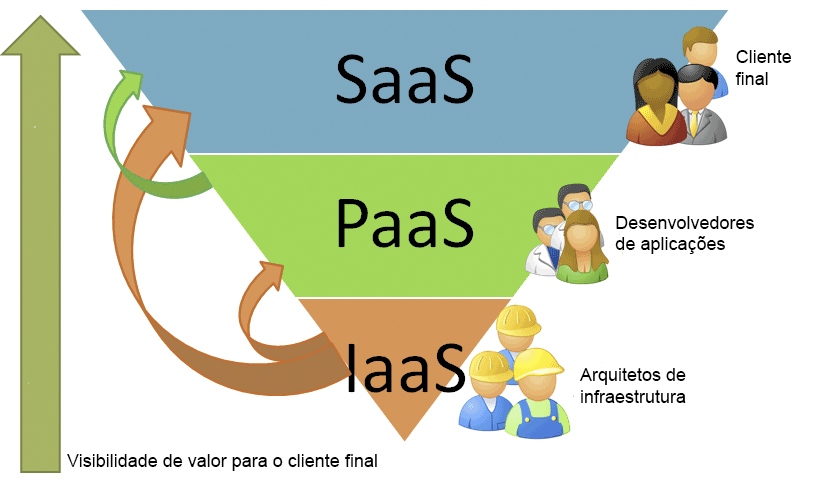
\includegraphics[scale=0.35]{imagem/piramide-cloud.png}
  \caption{Pirâmide representando os 3 serviços oferecidos por uma cloud}
  \label{img:piramide-cloud}
\end{figure}

\section{Virtualização}

Virtualização é a técnica que permite particionar um único sistema computacional em
vários outros, denominados máquinas virtuais \cite{virt-teoria-solucoes}. Segundo
este mesmo autor, estas máquinas virtuais oferecem um ambiente extremamente similar ao de uma máquina física.
Possuem seu próprio sistema operacional, aplicativos e serviços de rede. Ainda é possível
conectar um conjunto dessas máquinas virtuais através redes, switches ou roteadores virtualizados.

São diversas as tecnologias que implementam a virtualização de recursos computacionais.
Alguns dos mais conhecidos e evoluídos softwares desta área são: Hyper-V, Xen, KVM,
VMWare ESXi. \citeonline{virt-con-aplica} definem 3 partes básicas que podem ser
observadas em um ambiente de virtualização:

\begin{enumerate}
    \item
        O sistema nativo (real), conhecido também como sistema hospedeiro, que contém todo o hardware
        físico;

    \item
        O sistema virtual, conhecido também como sistema convidado, que executa o sistema virtualizado,
        simulando a maioria dos recursos de hardware que um sistema nativo poderia ter;

    \item
        A camada de virtualização, conhecida como \textit{hipervisor}, que faz a comunicação entre a
        interface virtual e nativa. Esta camada é representada pelos softwares de virtualização, como
        os já mencionados Hyper-V, Xen, KVM e VMWare ESXi.
\end{enumerate}

Este mesmo autor ainda diz que \emph{hipervisors} são mais complexos do que podem
parecer, por exemplo, caso o conjunto de instruções da máquina virtual e da real
sejam diferente (Linux virtualizado dentro de um Windows, ou vice-versa) haverá
a necessidade da conversão de instruções pela CPU da máquina real. É necessário
também mapear os recursos de hardware da máquina real (como mouses,
armazenamento externo, etc) que poderão ser acessados pela máquina virtual. Contudo,
todos os \emph{hipervisors} conhecidos já são extremamente evoluídos e lidam
muito bem com todas as complicações necessárias para possibilitar uma virtualização
adequada.

\citeonline{virt-teoria-solucoes} diz que é comum encontrarmos infra-estruturas com a filosofia de "um servidor
por serviço", por motivos de heterogeneidade das necessidades dos clientes e, alguns casos, até segurança. Normalmente, este
contexto acaba deixando o processador e alguns outros recursos subutilizados.

A virtualização resolve este problema de subutilização de recursos computacionais,
através do tratamento de ambas suas duas mais comuns causas: a filosofia ``um servidor por serviço'' e
a heterogeniedade das necessidades dos clientes.
Obtém-se diversos sistemas operacionais contidos em apenas um
hardware físico. Com uma máquina virtual disponibilizada para cada serviço, ela pode ter o sistema operacional,
bibliotecas e exatamente a configuração de memória, processador e armazenamento necessários para aquele serviço
funcionar, onde todos estes recursos podem ser inclusive alterados e dimensionados de acordo com o
crescimento ou decrescimento do consumo destes pelo serviço. Resumidamente, temos a flexibilidade, portabilidade,
um melhor aproveitamento dos recursos do hardware físico através do uso da quantidade adequada de máquinas virtuais e
elasticidade de executar diversos serviços diferentes, em sistemas operacionais diferentes, com necessidades de recursos
diferentes e que mudam conforme o tempo dentro, tudo dentro de um mesmo hardware. Este ato é conhecido como consolidação de servidores
e é imensamente importante para \textit{data-centers}, por exemplo, devido a diversas demandas de sistemas operacionais
por seus clientes, menor ocupação de espaço por máquinas físicas, melhor aproveitamento de energia elétrica, refrigeração, cabeamento, etc.

\section{Grid Computing}
\label{sec:grid}

Segundo \citeonline{foster1999grid}, o principal objetivo do
\textit{grid computing} é multiplexar recursos computacionais, de diversos provedores (hardware físico), de maneira
transparente para vários usuários. Desta maneira, o usuário percebe um único super-recurso, que na verdade é composto
por vários outros recursos menores.
\citeonline{grid-virtual-machines}, enunciam que, sistemas tradicionais de computação, por sua vez, multiplexam os
recursos de um único computador para vários usuários através da implementação de contas de usuários pelo
sistema operacional. Este modelo assume que existe uma entidade administrativa 100\%
confiável que possui permissão para adicionar usuários e restringir seu acesso conforme necessário. Enquanto isso,
sistemas de \emph{grid computing} devem possuir vários domínios diferentes, cada qual sua própria entidade administrativa, e não
podem depender de uma autoridade central.

\citeonline{grid-cloud-compared} nos mostram que a definição de \emph{cloud computing}
sobrepõe a de muitas tecnologias recentes, incluindo \emph{grid computing},
\emph{utility computing} e até \textit{web services} (estes dois últimos serão
devidamente mencionados nas duas próximas subseções). Segundo ele,
a definição de \emph{cloud computing} não só sobrepõe a de \emph{grid computing}, ela é de fato uma forma evoluída do
\emph{grid computing} e usa-o como base para seu funcionamento. Tal evolução teve como motivação a mudança do foco, que
antes era de infraestrutura para armazenamento e recursos de processamento, para recursos mais abstratos e serviços que apresentam um maior valor para seus usuários.

A sobreposição dos conceitos e a mudança de foco podem ser melhor entendidos visualizando a Figura \ref{img:grid-cloud-compared}.
Através dela, é evidente perceber que \emph{grid computing} é um conceito mais focado em aplicações e \emph{cloud computing} em serviços.
Pode-se notar também que \emph{clouds} utilizam \emph{grids} e que \emph{grids}, por sua vez, são baseadas \emph{clusters} de
computadores ou supercomputadores.

\begin{figure}[h]
  \center
  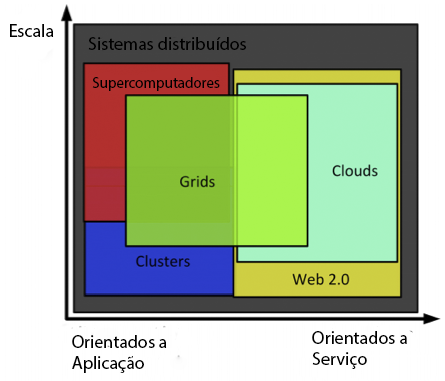
\includegraphics[scale=0.6]{imagem/grid-cloud-compared.png}
  \caption{Comparação de \emph{grid} e \emph{cloud computing}, mostrando a sobreposição dos conceitos}
  \caption*{Fonte: \citeonline{grid-cloud-compared}}
  \label{img:grid-cloud-compared}
\end{figure}

De acordo com \citeonline{grid-checklist}, a essência das definições do \emph{grid computing} pode ser capturada de
maneira simples em 3 itens:

\begin{enumerate}
    \item
        É composta por recursos coordenados que não dependem de um controle centralizado. Ela integra e
        coordena recursos e usuário de diferentes domínios de controle, por exemplo, diferentes unidades
        administrativas da mesma compania, ou até mesmo diferentes companias, cuidando de tudo que  diz
        respeito a segurança, políticas de acesso e qualquer outra configuração que venha a surgir de acordo
        com o contexto;

    \item
        Usa protocolos e interfaces padronizados, abertos e de propósito geral. Todos estes itens
        devem tratar problemas fundamentais, como autenticação, autorização, descoberta e acesso a
        recursos. É muito importante que estes protocolos e interfaces sejam abertos, caso contrário
        o sistema seria específico para determinada aplicação;

    \item
        Oferece uma qualidade de serviço não-trivial. Uma \emph{grid} permite que seus recursos sejam
        coordenados de maneira a entregar qualidades de serviço complexas, relacionadas a
        tempos de resposta, \textit{throughput}, avaliabilidade, segurança e co-alocação
        de múltiplos recursos para satisfazer as demandas de seus usuários. Assim, o sistema
        como um combinado tem uma utilidade maior que a soma de suas partes.

\end{enumerate}

\section{Utility Computing}

Segundo \citeonline{utility-market}, as técnicas tradicionais de gerenciamento de recursos
(alocação, controle de admissão e agendamento) se mostraram inadequadas para \emph{grids} compartilhadas,
definidas na Seção \ref{sec:grid}. Estas técnicas de gerenciamento de recursos não
fornecem facilidades para usuários requisitarem os recursos demandados de maneira apropriada e não refletem o valor,
importância e prazos da necessidade do usuário. Este problema ainda afeta diretamente os provedores
de \emph{grids} compartilhadas, já que não oferece nenhuma forma de seus contratantes serem compensados pelos recursos
compartilhados com outras entidades.

Não há como garantir que determinados usuários tenham acesso dedicado e com certos
níveis de qualidade de serviço e uma determinada gama de recursos, como processamento, memória e
armazenamento, não conseguindo extrapolar este limite. Pesquisadores e entusiastas encontraram
técnicas de gerenciamento de recursos baseadas no mercado que resolvem essas limitações. Tais
técnicas tem como objetivo fornecer um \emph{framework} para incentivar
os provedores de serviços priorizar a tarefas de maior importância, urgência e utilidade.
Este \emph{framework}, por sua vez, atua como \textit{middleware} em sistemas de \emph{grid computing}
garantindo que todos os conceitos de \emph{utility computing} sejam aplicados e respeitados
dentro daquele ambiente.

\begin{citacao}
    Existem muitas abordagens com relação ao \emph{utility computing}. Amplamente, elas se dividem
    em duas categorias. A primeira é o modelo de \textit{utilidade compartilhada}, onde
    os recursos são utilizados por diversos clientes ao mesmo tempo. A segunda, mais recente,
    é definida como modelo de \textit{utilidade de servidor completo}, onde aplicações
    programaticamente adquirirem e liberam o servidor conforme for necessário.
    \cite{utility-computing-models}
\end{citacao}

Para melhor entender as diferenças entre os modelos de utilidade compartilhada e
de servidor completo, temos a Figura \ref{img:utilidade-compartilhada}, demonstrando
um modelo de utilidade compartilhada. Nele, cargas de trabalho são entregues
a uma central de processamento, que irá distribuí-las entre vários servidores
(unidades de processamento compartilhado). Já para exemplificar o modelo de servidor
completo, temo a Figura \ref{img:utilidade-servidor-completo}: neste modelo,
aplicações são delegadas a um ou mais servidores exclusivos (de acordo com a
carga de processamento que esta aplicação necessita no momento), que processam nada
além destas aplicações a eles atribuídas.

\begin{figure}[h]
  \center
  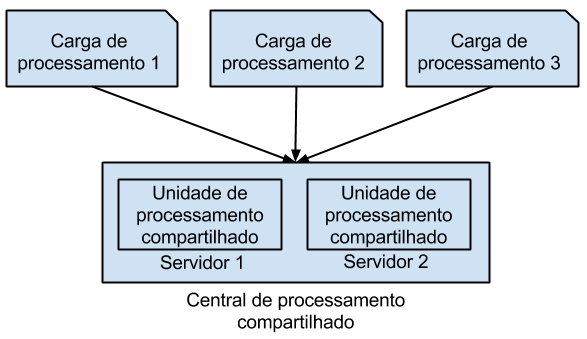
\includegraphics[scale=0.7]{imagem/utilidade-compartilhada.png}
  \caption{Modelo de utilidade compartilhada}
  \label{img:utilidade-compartilhada}
\end{figure}

\begin{figure}[h]
  \center
  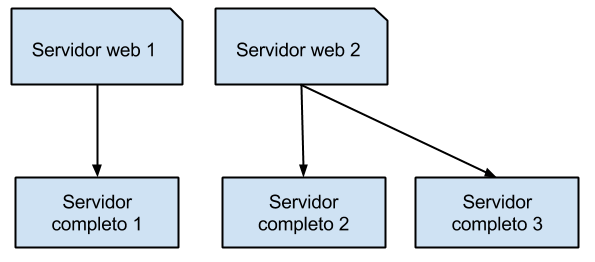
\includegraphics[scale=0.7]{imagem/utilidade-servidor-completo.png}
  \caption{Modelo de utilidade de servidor completo}
  \label{img:utilidade-servidor-completo}
\end{figure}

\section{Web Service}

\citeonline{web-services-distributed} definem
web services como: uma entidade programática que fornece uma funcionalidade particular, como
lógica de aplicação, e é disponibilizado para diversos potenciais usuários através da internet.
Segundo o mesmo, um grande conceito por trás dos \emph{web services} é o de arquiteturas orientadas
a serviços (\textit{service-oriented architecture}, em inglês, ou \emph{SOA}).
\textit{Web services} adicionaram um novo nível de funcionalidade para a atual \textit{Web},
tomando o primeiro passo em direção à integração de componentes de \emph{software} distribuídos
usando padrões da \emph{web} (protocolo HTTP, XML ou JSON, URIs, SOAP, WSDL, etc), definidos pela
\emph{World Wide Web Consortium} (W3C) \cite{book-web-services}.
Tal arquitetura sugere algumas atividades essenciais para o funcionamento dos determinados serviços, assim
como sua utilização por clientes (internos ou externos à organização desenvolvedora do serviço). São elas:

\begin{enumerate}
    \item
        Um serviço deve ser criado, com suas interfaces e métodos de chamada definidos;

    \item
        Ele deve ser publicado, seja em intranet ou internet, para que possíveis
        usuários possam localizá-lo;

    \item
        Deve ser localizável para que possa ser utilizado pelos potenciais usuários;

    \item
        O serviço precisa ser utilizado para que ofereça algum tipo de benefício;

    \item
        E o serviço preciso ser ``despublicado'', quando não é mais necessário ou não
        está mais disponível.
\end{enumerate}

Pode-se ver na Figura \ref{img:fluxo-webservice}, os passos necessários para que um
cliente possa finalmente utilizar um web service. Primeiramente, após construído, este
serviço (\textit{service provider}) deve ser publicado em um índice (chamado de \textit{service broker}).
Então, um cliente (\textit{service requester}), pode acessar o índice e procurar por um serviço
disponível para ele. Após este cliente acessar os dados do índice, ele se conecta diretamente com o
serviço e realiza a comunicação necessária para prosseguir com o uso deste.

\begin{figure}[h]
  \center
  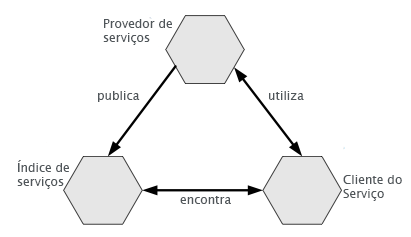
\includegraphics[scale=0.7]{imagem/fluxo-webservice.png}
  \caption{Fluxograma mostrando os passos para publicação, localização e uso de um web service}
  \caption*{Adaptado para português de \citeonline{web-services-distributed}}
  \label{img:fluxo-webservice}
\end{figure}

A comunicação baseada em tecnologias \emph{web} garante a interoperabilidade dos \emph{web
services}, independentemente plataforma em que é desenvolvido ou consultado.
Isto acaba ajudando equipes a desenvolver um software altamente escalável,
programando as partes mais custosas como serviços externos, usando as ferramentas
mais adequadas para que haja o esperado ganho em escalabilidade, ou em legibilidade do código.
Em um ambiente de \emph{cloud computing}, escalabilidade e interoperabilidade são
de suma importância para um aproveitamento eficiente dos recursos computacionais
disponíveis para esta finalidade e garantir o crescimento da \emph{cloud} sem problemas.
É evidente que manter uma parte de um \emph{software} isolada torna a manutenção e evolução
do seu código muito mais simples do que fazer o mesmo no \emph{software} completo, por inteiro.
Cada parte pode ser testada e finamente polida, ainda aproveitando das melhores
ferramentas que determinadas linguagens podem oferecer para a resolução de problemas
específicos.

  \chapter{Trabalhos relacionados}

São vários os trabalhos que já apresentam casos de sucesso de uso de diversos
modelos e tecnologias de cloud computing. Alguns dão enfoque a instituições de
ensino situadas em países em desenvolvimento, como o trabalho de
\citeonline{book-cloud-developing-countries}. Ele descreve a implantação
de cloud computing na Universidade de Tecnologia de Ho Chi Minh, no Vietnã,
para as tarefas de pesquisa e ensino.

No trabalho de \citeonline{book-cloud-developing-countries},
recursos fixos e pré-configurados deixaram de ser fornecidos,
em prol de recursos elásticos (que podem ser facilmente redimensionados)
e móveis (podem estar inclusive em lugares físicos diferentes de acordo com a
vontade do seu utilizador). Os pesquisadores forneciam os dados
relacionados aos recursos que precisavam, seja de hardware ou software, e em
segundos obtinham o devido acesso que necessitavam (IaaS). Eles também podiam
ter acesso simples e direto a plataformas para desenvolverem suas pesquisas da
maneira mais prática possível (PaaS). Além disso, foi criada uma rede social
para que os pesquisadores compartilharem informações científicas mais facilmente
entre eles.

Em resumo, \citeonline{book-cloud-developing-countries} nos dizem que
o cloud computing solucionou um grande problema da
universidade, que eram as diferentes necessidades de sistemas operacionais e softwares,
muitas vezes conflitantes, e a massiva manutenção manual demandada para a
instalação e configurações dos softwares adequados a cada um dos cursos. A cada
mudança nas necessidades de software de um determinado curso, era necessário que
este fosse instalado e devidamente configurado em cada máquina do laboratório,
tomando muito tempo e esforço.
Com \emph{cloud computing}, as máquinas dos laboratórios passaram a ser servidas
através de \emph{IaaS}, onde cada curso possui uma imagem
relacionada a ele, que cumpre todos os requisitos de software, hardware virtual
e sistema operacional necessários. Quando há alguma modificação nesses
requisitos, ela é feita diretamente na imagem e esta é novamente disponibilizada
para todos os terminais de acesso. Facilita-se assim o gerenciamento do
laboratório, eliminando uma boa parte do excesso de trabalho manual e ainda
agilizando todo o processo de manutenção dos recursos computacionais físicos e
de software.

Anteriormente, em outro trabalho, \citeonline{article-cloud-education-new-dawn}
apresentou um estudo de caso da
Universidade de Westminster, no Reino Unido. Com mais de 22 mil alunos, ela é
uma de várias universidades desse país que aderiu ao cloud computing. Tudo
começou quando o serviço de email desta instituição começou a ser abandonado por
parecer desatualizado. Através de pesquisas, foi descoberto que 96\% dos
estudantes desta universidade configuravam suas contas de email acadêmico para
automaticamente redirecionar os emails para uma conta externa
\cite{article-cloud-education-new-dawn}. Isto estava causando alguns problemas,
dentre eles: os emails começaram a ser tratados como \textit{spam} pelos emails
externos dos estudantes e, consequentemente, eles estavam deixando de receber
comunicados importantes; e os alunos acabavam frequentemente usando pendrives,
que são muito suscetíveis a perdas ou mal-uso, porque o serviço não fornecia
uma capacidade de armazenamento adequada.

Segundo este mesmo autor, para solucionar o problema, em 2007 a universidade
começou a estudar o \textit{Google Apps: Education Edition}. Através dele,
seriam oferecidos email com 7.3gb de armazenamento (o suficiente para os alunos
abandonarem o uso de pendrives), um sistema de troca de mensagens, calendário
compartilhado e até uma suíte de escritório com aplicações para processamento de
textos, planilhas e apresentações. Durante o ano 2009/9, após um determinado
período de testes e \textit{feedback}, o sistema foi implantado e os
problemas apontados foram mitigados com sucesso. Os estudantes passaram a ter
uma melhor experiência e a universidade estima uma economia de 1 milhão
de libras esterlinas, caso fosse fornecer um serviço semelhante de forma
independente.

Ainda há outros dois casos de uso em instituições de ensino mencionados por
\citeonline{article-cloud-education-new-dawn}. O primeiro, da Universidade da
Califórnia, nos Estados Unidos da América, que está usando cloud computing
para seu curso de desenvolvimento e implantação de aplicações SaaS
(\textit{software as a service}). Ajudada por uma doação da \textit{Amazon Web
Services} (AWS), todo o curso foi movido para a nuvem da empresa e eles podem
fornecer a grande quantidade de servidores que o curso demanda em apenas alguns
minutos \cite{site-cloud-education}. O segundo é o caso do Colégio de Medicina
do Centro de Biotecnologia e Bioengenharia de Wisconsin, que está usando os
servidores de cloud computing do Google para tornar pesquisas relacionadas a
proteínas, que costumam ser caríssimas, disponíveis para cientistas em todo o
mundo.

Contudo, as aplicações de \emph{cloud computing} já estudadas não se limitam
ao setor empresarial, de forma geral, e de ensino. \citeonline{federal-cloud-computing}
nos mostra estudos sobre a sua utilização no Governo Federal dos Estados Unidos.
Foi planejado investir 25\% do orçamento do governo (cerca de 20 bilhões de dólares)
para migração de sistemas de todas as suas agências para \emph{cloud computing}.
Para auxiliar tais agências neste processo foi elaborada a Estratégia Federal
de Cloud Computing, com o objetivo de:

\begin{itemize}
    \item
        expor benefícios, considerações e dilemas do \emph{cloud computing};
    \item
        fornecer um framework de decisões e alguns casos de uso de exemplo
        para ajudar as agências a migrarem seus sistemas;
    \item
        destacar recursos para sua implementação;
    \item
        identificar atividades, paéis e responsabilidades do governo federal
        para catalisar a sua adoção.
\end{itemize}

Então elaborou-se um paralelo entre as principais características do ammbiente atual
e do ambiente de \emph{cloud computing} proposto, segundo 3 critérios: eficiência,
agilidade e inovação, que pode ser visto na Tabela \ref{table:federal-cloud-computing}.
Todas as agências, antes de migrar seus sistemas, deveriam fazer este comparativo
aplicado a cada sistema específico a avaliar se esta migração oferecerá vantagens consideráveis.
É incluso neste trabalho o exemplo do Centro de Experiências do Exército (AEC), onde foi identificada
a necessidade de atualizar seu sistema de gerencimanto de relação com o cliente e após
considerarem diversas opções, como atualizar seu sistema proprietário de 10 anos de idade,
escolherem uma solução de \emph{software} como serviço disponível comercialmente. Esta
solução foi adaptada para todos os requisitos de segurança desta agência, proporcionava
todas as funcionalides que eram necessárias e foi entregue a uma fração do tempo
e dinheiro necessários para atualizar o antigo sistema legado. Durante o processo de escolha
chegou-se às seguinte conclusões sobre os critérios propostos:

\begin{itemize}
    \item
    Eficiência: o custo inicial de atualizar o sistema legado era de 500 mil a 1 milhão
    de dólares, enquanto o investimento inicial da solução de \emph{software} como serviço
    teve o custo de 54 mil dólares;

    \item
    Agilidade: foi considerado também o tempo para atualização do antigo \emph{software}.
    Apesar dos upgrades ao longo dos anos, era inviável customizá-lo com as necessidades
    do centro. Enquanto isso, a nova solução oferece provisiosamento em uma fração do tempo
    do seu antecessor, além de ser mais escalável e fácil de atualizar conforme o tempo;

    \item
    Inovação: a solução de \emph{software} como serviço integra-se diretamente
    com email e \emph{Facebook} e acesso a informação de qualquer lugar, através
    da \emph{internet} e permite a agência aproveitar do sistema de inovações
    do seu provedor de serviços sem ter que gerenciar pesados recursos computacionais.

\end{itemize}

\begin{table}
    \caption{Benefícios do Cloud Computing (Fonte: \cite{federal-cloud-computing})}
    \label{table:federal-cloud-computing}
    \centering
    \begin{tabular}{|p{8cm}|p{8cm}|}
        \hline
        \multicolumn{2}{|c|}{Eficiência} \\
        \hline
        Cloud Computing & Ambiente atual \\
        \hline
        \tabitem Alta utilização de recursos (maior que 60-70\%) & \tabitem Baixa utilização de recursos (menor que 30\%) \\
        \tabitem Demanda agregada e sistema acelerado de consolidação & \tabitem Demanda fragmentada e sistemas duplicados \\
        \tabitem Produtividade no desenvolvimento e gerenciamento de aplicações, redes e usuários finais & \tabitem Difícil gerenciamento \\
        \hline
        \multicolumn{2}{|c|}{Agilidade} \\
        \hline
        Cloud Computing & Ambiente atual \\
        \hline
        \tabitem Comprado como serviço de fornecedores confiáveis & \tabitem Requer anos para construção de data-centers para novos serviços \\
        \tabitem Incrementos e decrementos de capacidade quase instantâneos & \tabitem Requer meses para aumentar a capacidade de serviços existentes \\
        \tabitem Mais responsivo a necessidades urgentes \\
        \hline
        \multicolumn{2}{|c|}{Inovação} \\
        \hline
        Cloud Computing & Ambiente atual \\
        \hline
        \tabitem Muda o foco da posse dos recursos para gerenciamento de serviços & \tabitem Sobrecarregado com gerenciamento de recursos \\
        \tabitem Incentiva inovação no setor privado & \tabitem Totalmente desacoplado de inovações no setor privado \\
        \tabitem Encoraja uma cultura empreendedora & \tabitem Sem riscos, uso de tecnologia legada \\
        \tabitem Mais ligado a tecnologias emergentes \\
        \hline
    \end{tabular}
\end{table}

De acordo com o trabalho de \citeonline{ibm-cloud-computing}, a IBM, grande
empresa do ramo de computação, conhecida desde os seus primórdios, tem um caso
de uso de sucesso absoluto de \emph{cloud computing}. Na empresa, esta tecnologia
é utilizada dentro das 6 principais cargas de trabalho de tecnologia da informação:
desenvolvimento e testes, análise, armazenamento, collaboração, computação pessoal
e aplicações em produção. Graças a este uso, segundo estes mesmos autores, a
IBM melhorou sua eficiência, enquanto ao mesmo obteve impressivas economias em
capital e operações. O trabaho apresenta as seguintes considerações:

\begin{itemize}
    \item
        As equipes de desenvolvimento e testes presenciaram o tempo de provisionamento
        de um servidor cair de 5 dias ou mais para apenas uma hora. Isto impactou
        num acelerado desenvolvimento de novas funcionalidades e na velocidade
        com que as aplicações desenvolvidas chegavam no mercado;

    \item
        A nuvem de análise de dados melhorou incrivelmente a área de \emph{business intelligence},
        e reduziu os custos de projetos desta área, que eram da magnitude de centenas de milhares de dólares.
        As organizações que utilizam esta nuvem tem acesso a informação agregada de
        centenas de \emph{warehouses} (deposítos). Estas informações tem altíssimo valor, chegando
        a 300 milhões de dólares, somente para as 20 maiores consumidoras, de um total de 300 organizações.

    \item
        Sua central de armazenamento baseada em \emph{cloud computing} cortou
        o custo de armazenamento por \emph{byte} em 50\%, permitindo a IBM
        acomodar o grande crescimento de demanda por armazenamento (estimado
        em 25\% ao ano) sem aumentar o orçamento total destinado a essa área.

    \item
        A rede social \emph{IBM Connections}, hospedada em sua própria \emph{cloud},
        aumentao dramasticamente a colaboração entre seus funcionários e, consequentemente,
        a produtividade e inovação destes. Esta rede social suporta cerca de 50 milhões de minutos
        em conferência por mês.
\end{itemize}

Antes da implantação de tecnologias de \emph{cloud computing}, vários gárgalos
e problemas eram encontrados na IBM. Dentre estes problemas, por exemplo,
o setor de desenvolvimento e testes enfrentava semanas de espera para obter um
servidor, utilizava somente 10\% dele e não liberava seu uso devido ao tempo de
espera para obtê-lo novamente. Neste trabalho é apontado que 95\% do provisionamento
dos servidores é agora feito através de \emph{cloud}, confirmando sua velocidade e
facilidade de uso.

\citeonline{impact-cloud-computing} faz uma análise sobre o assunto e chega a conclusão que
os diversos serviços baseados em \emph{cloud computing} já disponíveis fizeram com que as
pessoas mudassem a maneira como pensam sobre conteúdo digital e como utilizá-lo.
No setor empresarial, a implantação de \emph{cloud computing} está aumentando constantemente,
independente do nicho. O crescimento de serviços que
podem ser oferecidos neste modelo de \emph{utility computing} continuará a mudar o mercado,
apresentar novos modelos de negócios e revolucionar a maneira como compartilha-se informações.

A Doutora Tua Huomo, em \citeonline{impact-cloud-computing}, diz que \emph{cloud computing}
não implica em apenas uma mudança de tecnologia, mas também forçará todos a adotarem
processos operacionais e de desenvolvimento que são mais focados no valor para
o cliente. Neste mesmo trabalho, o Professor Ian Biterllin prediz que qualidades
únicas desta nova tecnologia tornam-a muito mais amigável ao meio ambiente
do que todos os outros paradigmas conhecidos, mitigando as grandes críticas
recebidas por \emph{data centers} quando ao seu consumo energético. Finalmente,
o Dr Jonathan Liebanau, da Escola de Economia de Londres, em sua análise chega
à conclusão que \emph{cloud computing} trará diversas mudanças positivas na economia, porém
cada país sentirá essas mudanças com uma intensidade diferente: elas dependerão de como
os provedores de serviço, o governo e os diretores de empresas se adaptarão.

  \chapter{O Modelo Implementado}

Para implementar o ambiente de teste de \emph{cloud computing},
foi escolhida a pilha de ferramentas conhecida
como \emph{OpenStack}, implementada usando um nó para controle e \emph{networking}
da nuvem e outro nó para processamento. O modelo de rede escolhido para o ambiente
de testes foi o que é chamado pelo \emph{OpenStack} de \emph{simple flat networking},
onde apenas uma interface de rede é utilizada para todas as comunicações entre os serviços.
A instalação foi concebida com auxílio de
uma ferramenta de automação fornecida pela \emph{Rackpsace}, uma das empresas
criadores do próprio \emph{OpenStack} e uma das maiores do ramo de hospedagem
baseada em \emph{cloud computing}. Inicialmente, a intenção é de uma
nuvem privada, somente para uso interno da universidade. É esperada
uma evolução do projeto para uma nuvem híbrida, englobando também o conceito
de uma nuvem pública, para oferecer para empresas e outras insituições da região
os benefícios do \emph{cloud computing}.

\section{OpenStack}

O \emph{OpenStack} é um grupo de ferramentas, comumente chamado de ``ecossistema''
por sua comunidade desenvolvedora e utilizadora. Esse grupo é composto por
diversos serviços, são eles:

\begin{itemize}
    \item
        Keystone: serviço de autenticação entre os nós e serviços;

    \item
        Nova: serviço de processamento, que é responsável por distribuir,
        configurar e executar máquinas virtuais propriamente ditas;

    \item
        Glance: serviço responsável pela descoberta, registro e fornecimento
        de imagens de máquinas virtuais;

    \item
        Swift: serviço de armazenamento de objetos (arquivos), semelhante
        ao \emph{Amazon Simple Storage Service} (S3);

    \item
        Cinder: serviço de armazenamento de blocos, responsável por armazenar
        os discos virtuais utilizados pelas máquinas virtuais;

    \item
        Neutron: serviço de gerenciamento de redes virtuais, responsável
        por simular switches e roteadores e atribuir IPs às máquinas
        virtuais;

    \item
        Horizon: serviço de gerenciamento da nuvem. Fornece uma interface
        web para controle de tudo o que os outros serviços fornecem.
\end{itemize}

Pode-se observa como cada parte se comporta e com quem se comunica dentro do sistema
através da Figura \ref{img:openstack-services}.

\begin{figure}[h]
  \center
  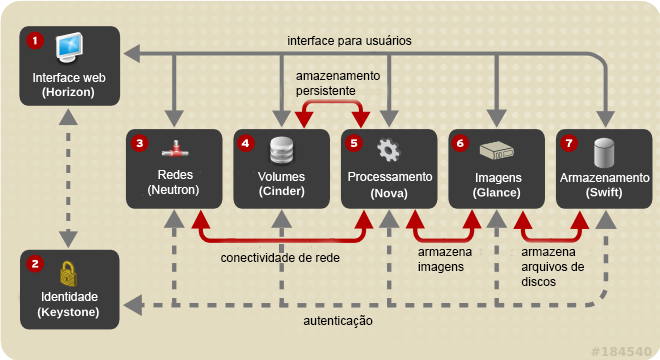
\includegraphics[scale=1.0]{imagem/openstack-services.png}
  \caption{Arquitetura do OpenStack}
  \caption*{Fonte: \url{https://access.redhat.com/documentation/en-US/Red_Hat_Enterprise_Linux_OpenStack_Platform/2/html/Getting_Started_Guide/ch01.html}}
  \label{img:openstack-services}
\end{figure}

Segundo \citeonline{rackspace-nasa-openstack}, este ecossistema foi fundado pela NASA e
pela \emph{Rackspace Hosting} e a partir de então teve uma grande adesão de
parceiros, tanto no meio científico quanto no meio corporativo. Um destes
grandes parceiros na área científica é o \emph{CERN} (Organização Europeia
para Pesquisa Nuclear), que analisa dados coletados pelo famoso \emph{LHC}
(Grande Colisor de Hádrons). \citeonline{cern-openstack} diz que
o \emph{OpenStack} é de grande importância dentro desta organização, fornecendo
recursos computacionais em larga escala para físicos espalhados pelo globo com
menos gargalos burocráticos.

Estes fatores, aliados às contribuições de diversos membros da comunidade de
software livre para uma rápida evolução do ecossistema foram essenciais para a
escolha destas ferramentas. Hoje, o projeto conta com novas versões a cada 6
meses, sempre incoporando diversas funcionalidades e implementando sugestões
de diversos usuários. A fundação do \emph{OpenStack} é composta por um comitê
técnico de 13 membros eleitos por contribuidores tecnológicos, um quadro de
24 diretores, sendo 8 apontados por membros, 8 eleitos por membros de classe e
8 eleitos por membros comuns, e por um comitê de usuários composto por mais de
75 grupos espalhados por todo o mundo.

\subsection{História}

Em 2008, os esforços da NASA para padronizar seus \emph{websites} inspiraram
uma explosão em tecnologias de \emph{cloud computing} \cite{nasa-cloud-computing}.
O projeto, em seu início, era chamado de \emph{NASA.net} e tinha como objetivo
unificar todas abordagens usadas para desenvolver tais \emph{websites}. Todos eles
pareciam diferentes e eram gerenciados de maneiras diversas. A idéia era
que os desenvolvedores pudessem criar seus \emph{websites}, enviá-los para o
\emph{website} do \emph{NASA.net} e ele tomaria conta de todos os passos necessários.

Apesar que o projeto estava apenas começando naquela época, seus desenvolvedores
já identificaram a necessidade de ter grandes ferramentas na sua fundação. O próximo
passo era construir um ``serviço de infraestrutura''. Foi criada então uma plataforma
capaz de fornecer poder computacional para rodar serviços da \emph{NASA.net} e que
também poderia ser usado para outros tipos de aplicações. O que a equipe de desevolvimento
percebeu foi que eles precisavam desenvolver um serviço de \emph{cloud computing}.
A idéia era se autenticar no serviço e dizer: preciso de 10 computadores e,
dentro de um minuto, ter acesso a estes 10 computadores para qualquer que seja
o propósito.

Conforme o escopo do projeto cresceu, ele foi renomeado para \emph{Nebula}. O \emph{Nebula}
estava fazendo muitos mais do que criar padrões para os desenvolvedores \emph{web}
da agência: era fornecida uma grande gama de serviços para desenvolvedores, pesquisadores,
e cientistas, para que eles pudessem acessar e gerenciar toda enorme quantidade de
dados que a NASA acumulava dia após dia.

Um dos pontos decisivos sobre o sucesso do \emph{Nebula}, antes de se tornar
oficialmente \emph{OpenStack} foi a escolha do modelo de \emph{software} livre.
\emph{Software} proprietário é tão útil e conveniente algumas vezes que a equipe
chegou a pensar se seria possível continuar o desenvolvimento do produto sem se
apoiar neste modelo. Por outro lado, o modelo de desenvolvimetno de código aberto facilitaria
um ambiente colaborativo: qualquer um com o conhecimento poderia melhorar o código. Esta
foi então a escolha, segundo O'Brien (um dos criadores e idealizadores da ferramenta),
desde o início era desejado que o projeto envolvesse uma grande comunidade (empresas
privadas, instituições acadêmicas e laboratórios de pesquisa, por exemplo) que
pudesse contribuir e levar o \emph{Nebula} a um nível mais alto.
O \emph{Nebula} acabou por evoluir e se tornar um projeto que estava atendendo
demandas e necessidades gerais, não somente da NASA, mas do mundo todo. Entretanto,
houve um problema com umas das partes do sistema, feita com software proprietário,
que precisava ser migrada para uma linguagem aberta. A linguagem escolhida foi Python, a
preferida da equipe de desenvolvimento.

A partir da publicação do \emph{Nebula} como \emph{software} livre, foi chamada
a atenção de diversos membros da indústria. Um deles, uma empresa de hospedagem
conhecida como \emph{Rackspace}, que também desenvolvia suas próprias
ferramentas para automatizar o processo de gerenciamento das aplicações
que seus clientes queriam hospedar, estava pronta para liberar suas próprias
ferramentas dentro do mesmo modelo de código aberto. Com a notícia, a Rackspace,
que tinha paixão por \emph{software} livre, entrou em contato com a equipe do \emph{Nebula}
para colaborar com o desenvolvimento do projeto. Um complementou o outro, e da
fusão dos dois projetos foi anunciado o \emph{OpenStack}, atraindo milhares de
colaboradores por todo o mundo e centenas de grandes empresas. Antes, o que
somente poderia ser feito pagamento para um terceiro, poderia ser então
feito de maneira totalmente gratuita, com uma ferramenta gratuita e aberta.

\subsection{Modelo de rede}

Uma das características mais complexas do ecossistema escolhido é a arquitetura
de rede. O ambiente de produção ideal deve fornecer 4 interfaces de rede para
total separação dos tráficos de gerenciamento, dos sistemas de armazenamento,
da rede privada das máquinas virtuais e da rede pública (que fornece IPs
flutuantes) e assim atingir o máximo de performance.

De acordo com a documentação do \emph{OpenStack}, é possível usar no mínimo duas interfaces de rede
com um \emph{switch} gerenciável, ou seja, capaz de roteamento de pacotes nas camadas 2 e 3
do modelo OSI, através de uma técnica conhecida como \emph{VLAN tagging} (\cite{l2-l3-vlan}). Também pode-se
chegar ao caso mais básico e simples: uma única interface de rede,
com o uso de um um nó de \emph{networking} (usando a ferramenta \emph{Neutron})
para desempenhar este papel, porém usando uma técnica conhecida como \emph{GRE} (Generic
Routing Encapsulation), que tem como desvantagem uma certa lentidão
para o encapsulamento dos pacotes e gera um gargalo na inteface de rede deste
nó (todo tráfego precisa passar por ele).

Para este ambiente de testes, logicamente, foi usado o modelo de rede mais
simples, conhecido como \emph{simple flat networking}, dada a facilidade
de implementação deste utilizando a ferramenta Neutron e a técnica \emph{GRE}.

\subsection{Configuração e instalação}

Foram realizadas diversas tentativas de instalação e configuração do projeto
utilizando os manuais do próprio \emph{OpenStack}, disponíveis na documentação
oficial, porém sem sucesso. São diversas configurações espalhadas por arquivos
diferentes e diversos comandos extremamente sensíveis. Se um erro é cometido,
ele só será notado quando todas as ferramentas do ecossistemas forem instaladas
e implicará em uma análise de \emph{logs} para futura correção. Como solução
para este problema, o próprio projeto recomenda o uso de ferramentas de automação,
sendo as mais conhecidas: \emph{Salt}, \emph{Puppet} e \emph{Chef}.

Para o desenvolvimento deste ambientes de testes, foi escolhida a ferramenta
\emph{Chef}, usada com scripts fornecidos pela própria Rackspace, por causa
do excepcional suporte oferecido pela empresa, tanto para o seu uso quanto para
toda a configuração necessária, através do programa \emph{Rackspace Private Cloud}.
Durante todo o processo (que será descrito abaixo), diversos problemas na ferramenta de automação
fornecida pela Rackspace foram encontrados e reportados à equipe de desenvolvimento,
que rapidamente corrigiu-os para que fosse possível continuar o procedimento.
O programa \emph{Rackspace Private Cloud} compreende um pacote de \emph{software livre} para a instalação do
\emph{OpenStack}, treinamento e certificação, prestação de serviços e opções
de suporte para auxiliar a construção e gerenciamento da nuvem privada. Como
eles possuem a maior infraestrutura baseada no \emph{OpenStack} do mundo, há possibilidade
de acesso aos profissionais que participaram deste grande feito e enfrentaram os
mais diversos problemas para tal infraestrutura.

O \emph{Chef} é uma ferramenta de automação e gerenciamento de infraestrutura
baseada no modelo cliente-servidor. Tarefas para controle de infraestrutura,
chamadas de de \emph{recipes} (receitas), definem instruções
para instalar e configurar bancos de dados, servidores web e balanceadores de
carga, por exemplo. Estas receitas, por sua vez, são compostas de \emph{resources}
(recursos), como um arquivo, um \emph{template} ou um pacote do sistema a ser instalado.
Há também a possibilidade de agrupar receitas em \emph{roles}, ou papéis, para
uma maior abstração da infraesturura, permitindo que diversas receitas sejam
executadas em múltiplos nós. Todas as receitas e papéis são armazenados no servidor
(\emph{chef-server}) e os clientes se registram e sincronizam-se através do
\emph{chef-client}. A partir deste ponto, ao comando do servidor, os próprios
clientes executam as receitas das dos papéis atribuitdos a eles em si mesmos. Para
configuração tanto do chef-server quando dos nós que serão provisionados através
do \emph{chef-client}, existe a ferramenta \emph{knife}. Ela que envia o \emph{cookbook}
(conjunto de receitas) para o chef-server e faz o registro dos \emph{chef-clients}
neste servidor. Tal ferramenta pode ser instala no próprio \emph{chef-server} ou em
outro computador, conforme necessidade e conveniência. Veja a Figura \ref{img:chef}
para uma melhor compreensão da organização e comunicação deste conjunto.

\begin{figure}[h]
  \center
  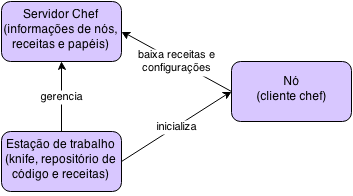
\includegraphics[scale=1.0]{imagem/chef.png}
  \caption{Fluxograma de funcionamento do Chef}
  \label{img:chef}
\end{figure}

Finalizando, para o ambiente de testes foram utilizados 4 computadores
e um pequeno roteador, cedidos pelo Laboratório Ada Lovelace, do curso de
Ciência da Computação da UENF. Cada um dos computadores possui a seguinte configuração:

\begin{itemize}
    \item Processador: Core i5 de segunda geração, com 4 núcleos rodando a 3.4 Ghz;
    \item Memória: 4GB DDR3 1066 Mhz;
    \item Disco rígido: HDD 160GB 7200rpm.
    \item Sistema Operacional: Ubuntu Server 12.04 64 bits
\end{itemize}

Um deles foi configurado para ser o \emph{chef-server}, um para ser o nó controlador
da nuvem e um nó para processamento das máquinas virtuais. Basicamente, o processo de
instalação consiste nos seguintes passos:

\begin{enumerate}
  \item Preparação do nós (instalação de sistema operacional)
  \item Instalação do \emph{chef-server}, dos livros de receitas da Rackspace
  \item Criação de um ambiente \emph{chef} e definição dos seus atributos (configurações)
  \item Instalação do \emph{chef-client} nos nós
  \item Atribuição e aplicação dos papéis aos nós controlador, de rede e de
    processamento
\end{enumerate}

Como a preparação dos nós é aberta para ser feita de acordo com o costume do usuário,
bastando que seja instalado o sistema operacional indicado, este passo não será
descrito.

\subsubsection{Instalação do chef-server e livros de receitas
da Rackspace}

Após preparar os nós, escolhe-se um para ser o \emph{chef-server} e então,
logado como o usuário \emph{root}, instala-se o software com os comandos mostrados
no Código \ref{cod:chef-server-install}

\begin{listing}
\begin{minted}[frame=lines,framerule=2pt]{bash}
  $ curl -s -O https://raw.githubusercontent.com/rcbops/support-tools/
  master/chef-install/install-chef-server.sh
  $ bash install-chef-server.sh
\end{minted}
\caption{Instalação do \emph{chef-server}}
\label{cod:chef-server-install}
\end{listing}

Após este processo terminar, recarrega-se o terminal para atualizar as variáveis
necessárias e testa-se o comando \emph{knife} através dos comando no Código \ref{cod:test-chef}.

\begin{listing}
\begin{minted}[frame=lines,framerule=2pt]{bash}
  $ source /root/.bash_profile
  $ knife client list
\end{minted}
\caption{Teste de instalação do \emph{chef}}
\label{cod:test-chef}
\end{listing}

A instalação dos livros da receitas da Rackspace é feita através dos seus repositórios
de código, seguindo os comandos do Código \ref{cod:chef-cookbooks}.

\begin{listing}
\begin{minted}[frame=lines,framerule=2pt]{bash}
  $ git clone https://github.com/rcbops/chef-cookbooks.git
  $ cd chef-cookbooks
  $ git checkout 4.1.2
  $ git submodule sync
  $ git submodule update
  $ knife cookbook upload -a -o cookbooks
  $ knife role from file roles/*rb
\end{minted}
\caption{Instalação dos livros de receitas da Rackspace}
\label{cod:chef-cookbooks}
\end{listing}

\subsubsection{Criação do ambiente para configuração do OpenStack}

A partir dai é iniciada a parte de criação do ambiente no \emph{chef} e
configuração das variáveis do \emph{OpenStack} em si. Para criar o ambiente e
abrir o arquivo de configuração, executa-se os comandos apresentados no Código
\ref{cod:knife}.

\begin{listing}
\begin{minted}[frame=lines,framerule=2pt]{bash}
  $ knife environment create private-cloud -d "UENF Private Cloud"
  $ knife environment edit private-cloud
\end{minted}
\caption{Criação do ambiente do \emph{chef}, visualização e edição das variáveis
 deste ambiente}
\label{cod:knife}
\end{listing}

Ao executar o último comando, será aberto o arquivo em branco, onde deve-se
sobrescrever as variáveis padrões definidas pela Rackspace de maneira
adequada à infraestrutura onde o sistema está sendo configurado. Como mencionado
anteriormente, o modelo de rede é complicado, tomando um tempo considerável para
sua compreensão e o fato de haver somente uma interface de rede para o ambiente
de testes adicionou uma complexidade extra ao processo. A equipe de suporte
da Rackspace teve que ser acionada para auxiliar o processo de configuração.
A partir dai, o arquivo de configuração ideal para a implantação do ambiente
de teste foi estabalecido como mostrado no Código \ref{cod:json}. Nesta imagem
pode-se observar no atributo \emph{osop\_networks} que as 3 redes utilizadas
pelo \emph{OpenStack} estão configuradoas sob a mesma faixa de IPs, ou seja,
todas elas na mesma interface de rede.

\begin{listing}
\begin{minted}[frame=lines,framerule=2pt]{javascript}
{
  "name": "rpcv412",
  "description": "Rackspace Private Cloud v4.2.2",
  "cookbook_versions": {
  },
  "json_class": "Chef::Environment",
  "chef_type": "environment",
  "default_attributes": {
  },
  "override_attributes": {
    "nova": {
      "libvirt": {
        "vncserver_listen": "0.0.0.0"
      },
      "network": {
        "provider": "neutron"
      }
    },
    "neutron": {
      "ovs": {
        "provider_networks": [
          {
            "label": "ph-eth0",
            "bridge": "br-eth0",
            "vlans": "1:1"
          }
        ],
        "network_type": "gre"
      }
    },
    "mysql": {
      "allow_remote_root": true,
      "root_network_acl": "%"
    },
    "osops_networks": {
      "nova": "192.168.0.0/24",
      "public": "192.168.0.0/24",
      "management": "192.168.0.0/24"
    }
  }
}
\end{minted}
\caption{Arquivo de configuração das variáveis utilizadas para o ambiente de testes
montado}
\label{cod:json}
\end{listing}

\subsubsection{Instalação do chef-client nos nós da cloud}

Para a configuração do \emph{chef-client} nos nós onde os componentes do \emph{OpenStack}
serão instalados, é necessária a criação de uma chave SSH para conexão sem senhas e depois
proceder a instalação usando a ferramenta \emph{knife bootstrap}, como visto no Código
\ref{cod:knife-bootstrap}, substituindo \emph{\textless usuario\textgreater} e
\emph{\textless ip\textgreater} pelo usuário e IP
de cada nó que se deseja adicionar ao ambiente.

\begin{listing}
\begin{minted}[frame=lines,framerule=2pt]{bash}
$ ssh-keygen
$ knife bootstrap -E private-cloud -i .ssh/id_rsa_private --sudo
-x <usuario> <ip>
\end{minted}
\caption{Código para realizar a configuração do \emph{chef-client} nos nós do ambiente}
\label{cod:knife-bootstrap}
\end{listing}

Após o processo terminar, é necessário que cada nó da rede possa acessar o
\emph{chef-server} pelo \emph{hostname}. Para isto, adiciona-se uma linha
para cada nó no arquivo \emph{/etc/hosts} seguindo o seguinte modelo do Código
\ref{cod:hosts}. A partir daí, o registro do nó cliente com o \emph{chef-server} é feito
executando-se comando \emph{chef-client}.

\begin{listing}
\begin{minted}[frame=lines,framerule=2pt]{text}
<ip-chef-server> <hostname-chef-server>
\end{minted}
\caption{Modelo de arquivo de configuração de \emph{hosts} nos nós clientes}
\label{cod:hosts}
\end{listing}

\subsubsection{Atribuição e aplicação dos papéis aos nós}

Prossegue-se então com a atribuição dos papéis aos nós que farão parte da
\emph{cloud}. Como dito anteriormente, para o ambiente de teste foram usados
um nó controlador, um de rede e um de processamento. São executados os comandos
mostrados no Código \ref{cod:role} em cada nó, substituindo o \emph{\textless papel\textgreater}
por \emph{role[ha-controller]}, \emph{role[single-compute]} e \emph{role[single-network]}
e \emph{\textless hostname\textgreater} pelo \emph{hostname} deste mesmo nó.

Ao fim do procedimento, o \emph{OpenStack} já deve estar acesível através do
painel Horizon através do IP do nó controlador. A autentição pode ser feita
com o usuário \emph{admin} e a senha \emph{secrete}. Estas credenciais podem
ser modificadas a qualquer momento e outras mais também podem ser criadas.

Pode-se adicionar mais nós de rede e processamento de máquinas virtuais
conforme necessário, repetindo os processos de preparação do nó a ser adicionado,
instalação do \emph{chef-client} (Código \ref{cod:knife-bootstrap}),
configuração do arquivo de \emph{hosts} (Código \ref{cod:hosts}), atribuição
do papel (Código \ref{cod:role}) e execução do comando \emph{chef-client} no
próprio nó.

\begin{listing}
\begin{minted}[frame=lines,framerule=2pt]{bash}
$ knife node run_list add <hostname> '<papel>'
\end{minted}
\caption{Comando para atribuit um papel a um nó}
\label{cod:role}
\end{listing}

  \chapter{Resultados e discussões}
\label{cha:conclusoes}

Após todos os passos serem seguidos e os servidores devidamente configurados,
iniciaram-se os testes do \emph{OpenStack} para avaliar sua facilidade de uso,
performance e funcionalidades, colocando em julgamento também integração
com ferramentas para maiores abstrações (PaaS e SaaS) e o ciclo de desenvolvimento
do projeto.

\begin{figure}[h]
  \center
  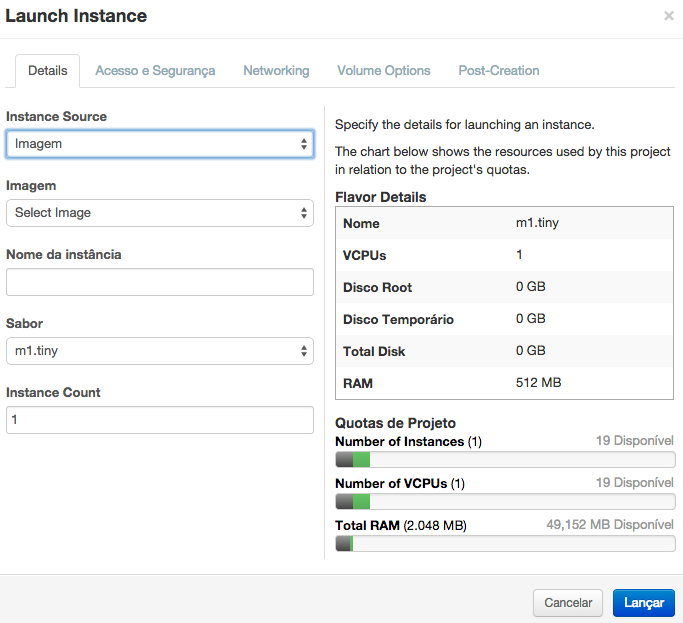
\includegraphics[scale=0.4]{imagem/criar-instancia-detalhes.png}
  \caption{Detalhes da nova instância a ser criada}
  \label{img:criar-instancia-detalhes}
  \center
  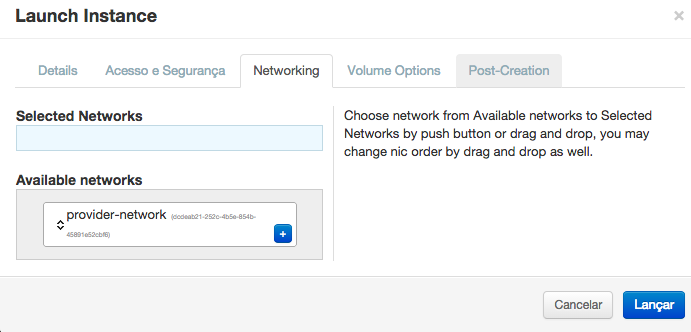
\includegraphics[scale=0.4]{imagem/criar-instancia-redes.png}
  \caption{Configurações de rede de uma nova instância}
  \label{img:criar-instancia-redes}
\end{figure}

A interface \emph{web} para gerenciamento das máquinas virtuais é extremamente simples,
desde a criação até a alteração dos recursos computacionais destas, atingindo
as expectativas com relação a este quesito. É possível definir vários ``sabores'' de máquinas
virtuais com configurações fixas de processador, armazenamento, memória e rede
(vide Figuras \ref{img:criar-instancia-detalhes} e \ref{img:criar-instancia-redes}).
Estas máquinas são criadas baseadas em imagens enviadas para o sistema e podem
ser ligadas e volumes persistentes de armazenamento para compartilhamento e
consolidação (agrupamento) de dados, como mostra a Figura \ref{img:criar-instancia-volume-site}.
Há também a  possibilidade de fazer um \emph{snapshot} (imagem) de um determinado servidor
para posterior restauração ou duplicação, criando outro servidores a partir deste
mesmo \emph{snapshot} (ver Figura \ref{img:imagens-e-snapshots}).

\begin{figure}[h]
  \center
  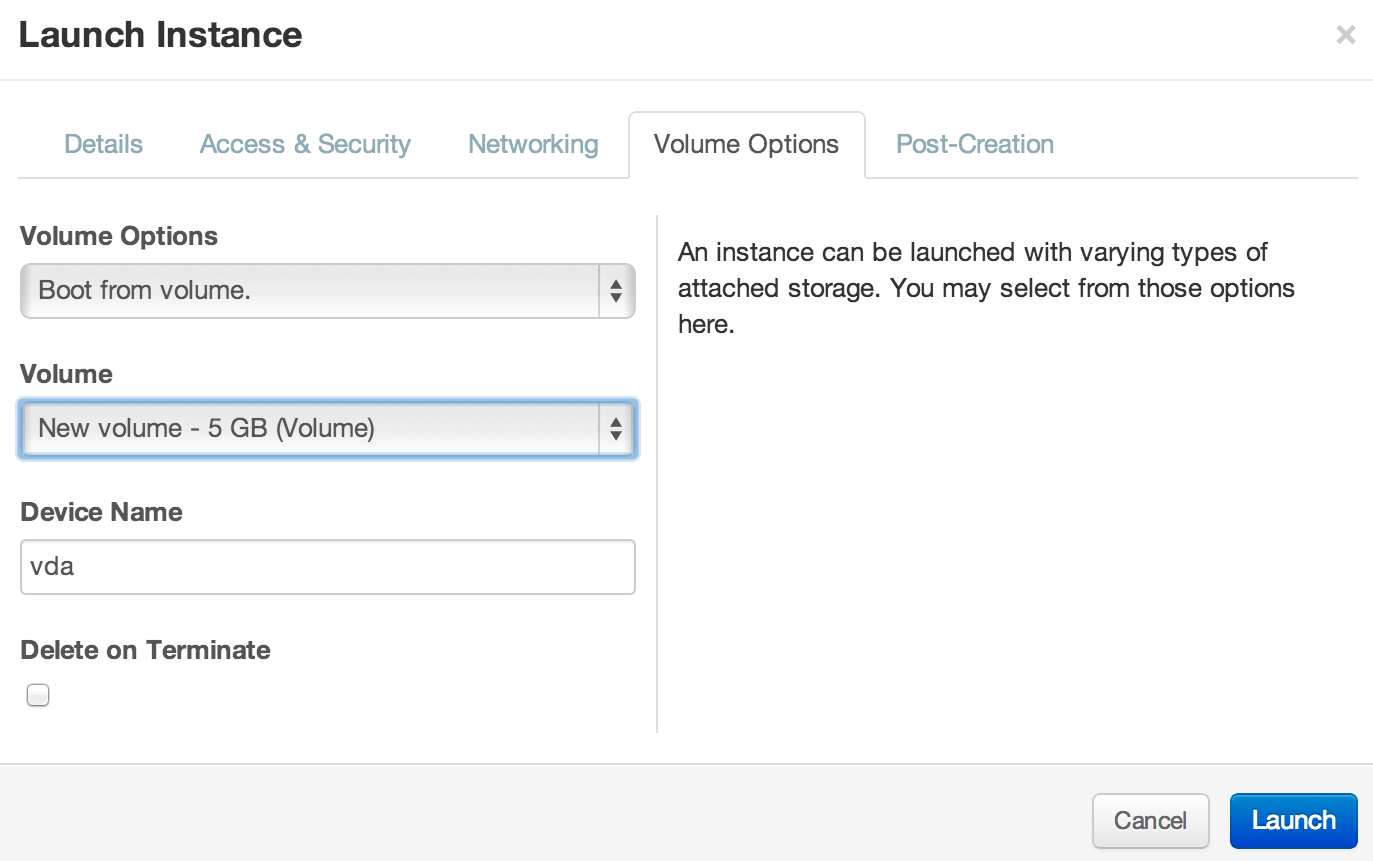
\includegraphics[scale=0.50]{imagem/criar-instancia-volume-site.png}
  \caption{Configurações de volume da nova instância}
  \label{img:criar-instancia-volume-site}
\end{figure}

\begin{figure}[h]
  \center
  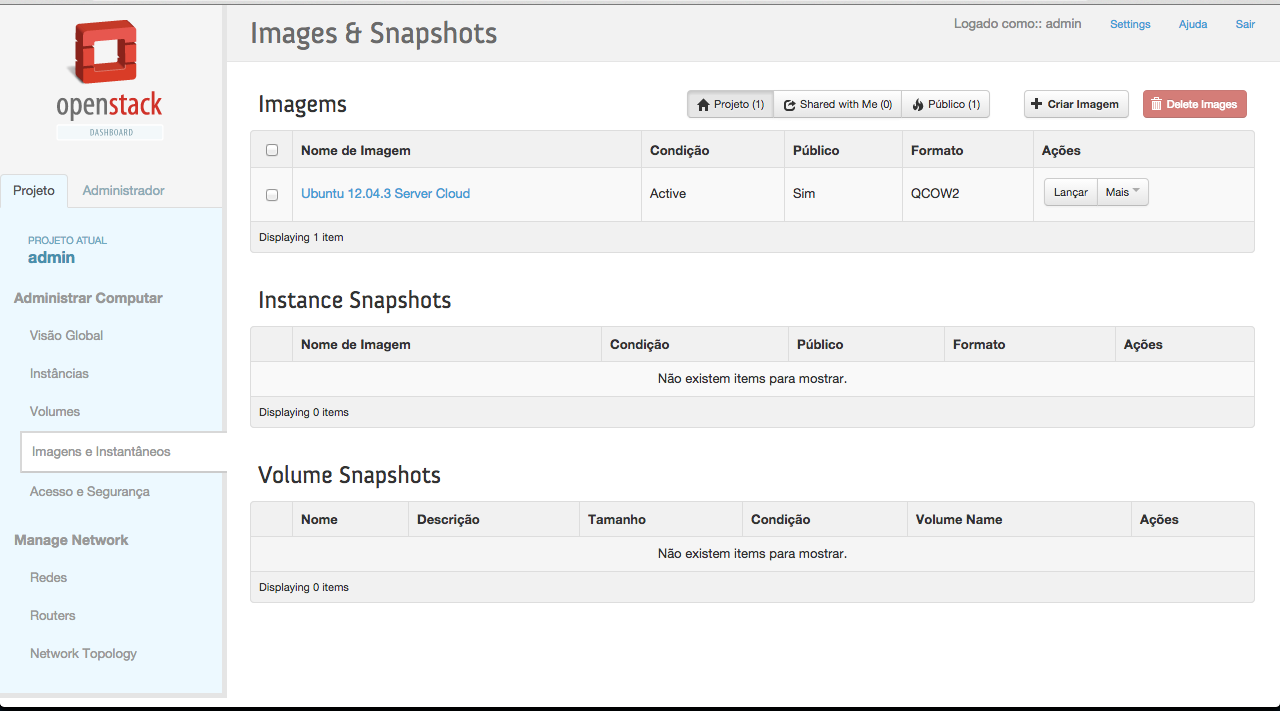
\includegraphics[scale=0.3]{imagem/imagens-e-snapshots.png}
  \caption{Interface para gerenciamento de volumes persistentes e snapshots}
  \label{img:imagens-e-snapshots}
\end{figure}

Existe também o controle de acesso e segurança das instância, onde são criados
usuários para o sistema. Cada usuário pode ter uma chave de criptografia, que será
usada para autenticá-lo com os servidores que tiver autorização de acesso e
fornecer um canal seguro de comunicação entre eles, como poder ser visto na
Figura \ref{img:acesso-e-seguranca-chaves}. Na área mostrada na Figura
\ref{img:acesso-e-seguranca-grupos-site} são
configuradas quais portas de cada servidor que aceitarão conexões de entrada.
Nesta seção, ilustrada pela Figura \ref{img:acesso-e-seguranca-acesso-api} é
possível também visualizar todos os pontos de acesso dos serviços
do \emph{cluster}, assim como as credenciais para acesso a eles.
Existe um \emph{super admin} capaz de utilizar esta interface para criar
\emph{tenants}\footnote{conceito utilizado para isolar dados de diferentes clientes
em um só sistema de uma maneira segura e eficiente}.
no \emph{OpenStack}, permitindo que diversas organizações utilizem o sistema sem
conhecimento e interferência entre si e com suas prórias regras individuais de
segurança.

\begin{figure}[h]
  \center
  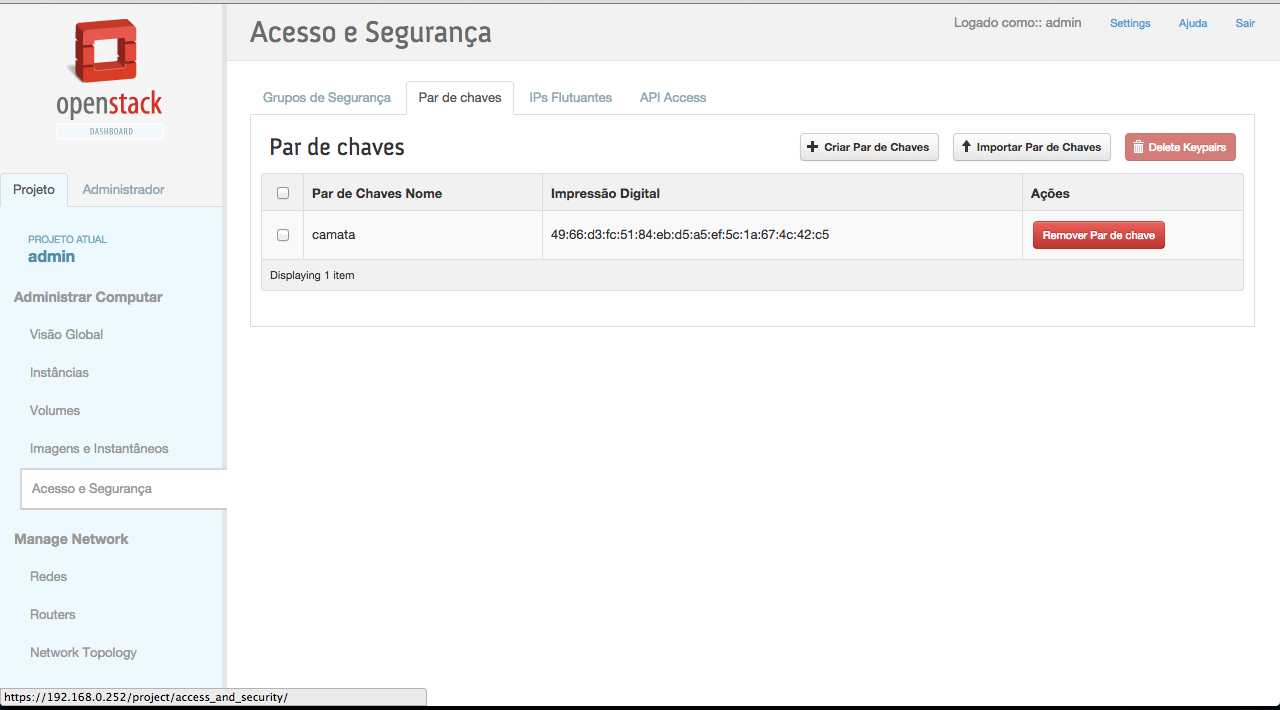
\includegraphics[scale=0.3]{imagem/acesso-e-seguranca-chaves.png}
  \caption{Interface para criação e visualização das chaves de acesso às máquinas
 virtuais}
  \label{img:acesso-e-seguranca-chaves}
\end{figure}

\begin{figure}[h]
  \center
  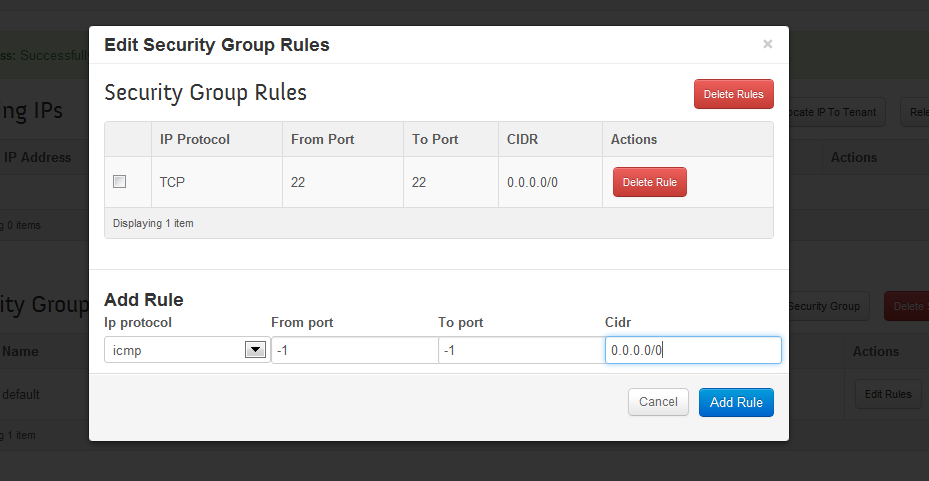
\includegraphics[scale=0.6]{imagem/acesso-e-seguranca-grupos-site.png}
  \caption{Configurações de permissões de rede de grupos}
  \label{img:acesso-e-seguranca-grupos-site}
\end{figure}

\begin{figure}[h]
  \center
  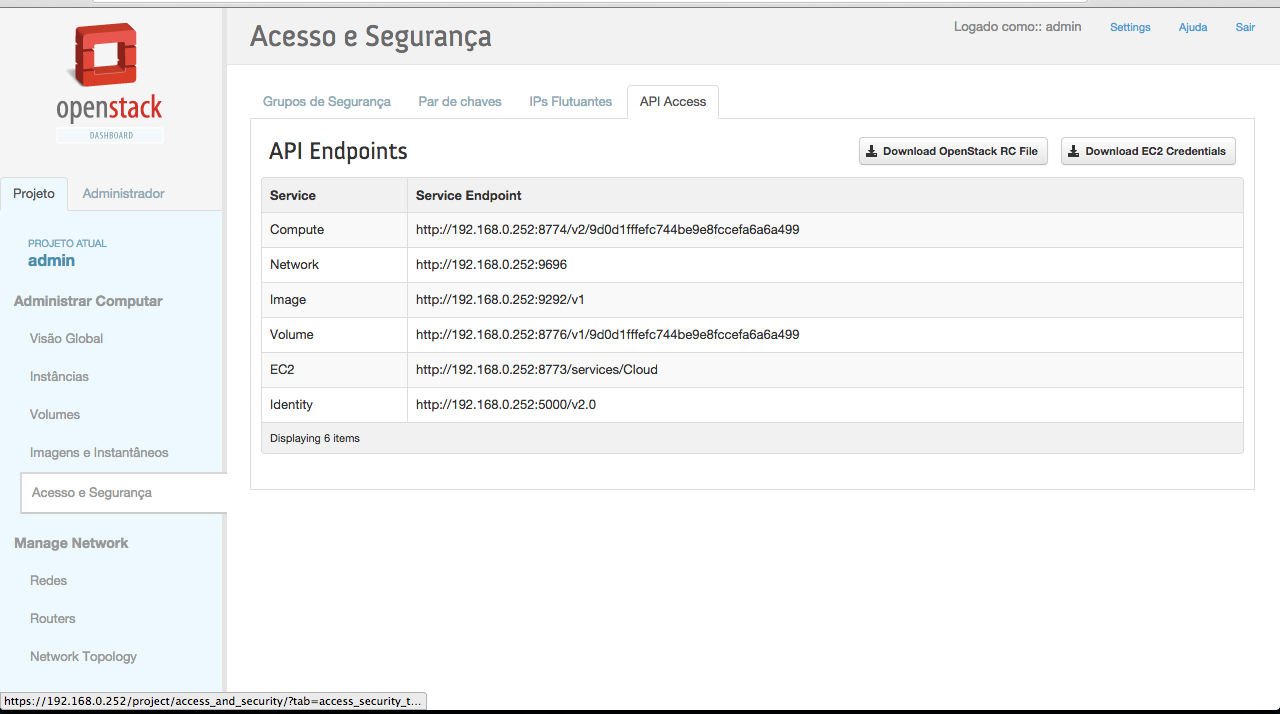
\includegraphics[scale=0.3]{imagem/acesso-e-seguranca-acesso-api.png}
  \caption{Visualização de \emph{URLs} de serviços e credenciais de acesso}
  \label{img:acesso-e-seguranca-acesso-api}
\end{figure}

Durante o desenvolvimento deste experimento, não havia uma ferramenta dentro do
\emph{OpenStack} para alcançar o nível de \emph{PaaS}: apenas ferramentas
desenvolvidas por terceiros (como o Juju, da Canonical, e o Tsuru, da Globo.com)
forneciam essa funcionalidade através das ricas APIs expostas pelo \emph{OpenStack}.
Contudo, antes mesmo do fim do experimento, foi desenvolvida e integrada uma
ferramenta para esta funcionalidade no projeto, chamada de \emph{Heat}, que não
foi considerada nesta análise devido à falta de tempo hábil.

Através de todas estas características, uma conclusão é eminente: o processo
de aquisição de infraestrutura computacional no paradigma de \emph{cloud computing}
é extremamente mais rápido e prático do que no modelo tradicional. Não bastante
esta vantagen, cada usuário pode se servir e adquirir a quantidade de recursos
necessários ao seu projeto e expandir ou diminuir conforme necessário (a interface
mostrada na figura \ref{img:criar-instancia-detalhes}, é também utilizada para a
edição das máquinas já criadas dentro do sistema. Além disso,
a interface é extremamente simples, possibilitando que qualquer pesquisador ou aluno
tenha acesso à infraestrutura que precisar para atingir seu objetivo, melhorando
ensino, pesquisa e também a própria universidade. Chegamos
então ao principal ponto econômico: graças a essa elasticidade, de uso e liberação
dos recursos, o \emph{cloud computing} oferece uma grande economia, evitando
o desperdício através de recursos escassos e fragmentados, favorecendo
ainda mais o melhoramento dos recursos computacionais da própria instituição.


% Também é um objetivo deste trabalho fazer uma
% discussão mais profunda sobre os detalhes técnicos da instalação
% do modelo, prover instruções para este processo, analisar as características do produto resultante
% e do processo, como um todo, verificar o nível do desenvolvimento do conjunto de ferramentas escolhido.

  \chapter{Conclusões}
\label{cha:conclusoes}

Pode-se concluir através das análises da bibliografia, das tecnologias e das
ferramentas apresentadas que \emph{cloud computing} é extremamente eficaz em
um ambiente acadêmico. Professores podem ter um rápido acesso a infraestrutura
para poder executar e/ou disponibilizar seus projetos, e alunos para auxílio
na instalação e configuração de ambientes para o aprendizado das mais diversas
tecnologias disponíveis, sem toda a burocracia já conhecida das instituições
públicas de ensino superior
(um servidor pode ser entregue em questão de minutos, em vez de dias, ou até mais),
Isto soluciona o problema alunos do curso de Ciência da Computação, que poderão
instalar seus aplicativos em máquinas virtuais isoladas, sem interferir uns nos
outros e ter que lidar com sistema operacional ``congestionado'' por ter diversos
\emph{softwares} diferentes instalados.
Além disso, toda a arquitetura obtida desta maneira possui um grande potencial
elástico e pode ser manipulada por uma interface web simples, intuitiva, poderosa
e eficaz para que os recursos sejam redimensionados conforme a necessidade do usuário.
É oferecida uma economia para a instituição de ensino, que através da
distribuição dos servidores virtuais nos físicos e seu uso sob-demanda, tem um
melhor proveito dos mesmos. Todas estas conclusões confirmam que os problemas
encontradas pela UENF com a gerencia de seus recursos computacionais podem
ser solucionados inteligentemente e oferecer vantagens para diversos alunos
e professores da universidade.

É visto que a instalação e configuração do próprio \emph{OpenStack} e das
ferramentas que é compõe tem sua complexidade concentrada no modelo de rede:
existem diversas ferramentas de automação que realizam todo processo de instalação
e configuração de pacotes Linux nos servidores de maneira automática e bem
transparente. A Rackspace oferece um ótimo suporte gratuito para auxiliar em
algumas tarefas e tem um completo time experiente em grandes ambientes de
\emph{cloud computing} para consultorias e outros serviços pagos relacionados
a escalabilidade e manutenção dos recursos computacionais necessários, o que é
de suma importância.

Foi constado que a ferramenta está evoluindo em velocidade crescente, com cada
vez mais recursos sendo integrados e desenvolvidos pelos contribuidores do projeto.
Somente durante o desenvolvimento deste trabalho, duas novas versões foram lançadas,
ambas adicionando novas funcionalidades para suprir as necessidades dos seus
usuários. Isto tudo é permitido graças ao desenvolvimento no modelo de software
livre, onde todos podem contribuir com o projeto.

\section{Trabalhos futuros}
\label{sec:trabalhos_futuros}

Este trabalho deixa inúmeros assuntos interessantes para trabalhos futuros, como
uma análise de ferramentas capazes de levar a \emph{cloud} para o nível de
plataforma como serviço (usando ferramentas como as já mencionadas Juju e Tsuru).
Tal serviço é de extrema utilidade para desenvolvedores de aplicações que não
tem conhecimento de gerenciamento de servidores e torna esta tarefa extremamente
simples, rápida e prazerosa. Também seria de grande contribuição uma análise
de performance de diferentes \emph{hypervisors}, elaboração de ambientes de
alta disponibilidade de nós controladores, de processamento e de volumes.

Um importante trabalho futuro sequencial a este projeto está sendo elaborado no
momento. Servidores e equipamentos de rede de alta performance foram adquiridos
pela universidade através de um edital de apoio da FAPERJ para que a \emph{cloud}
seja disponibilizada para ser utilizada pelos próprios alunos e professores da
UENF. O uso inicial deste equipamento abrange oferecer hospedagem e ambiente
de testes para aplicações desenvolvidas pelos próprios alunos do curso de Ciência
da Computação, através de bolsas de iniciação científica e tecnológica.


  % \anexo
  % \input{tex/anexo_efetividade_tdd}
  % \input{tex/anexo_codigos_do_comparativo}

  %--------------------------------- Bibliografia ------------------------------

  \citeoption{abnt-repeated-author-omit=yes}
  \bibliographystyle{abnt-alf}
  \bibliography{bibliografia}
\end{document}
